\section{Implementierung und Deployment}
\subsection{Technologieauswahl und Implementierungsdetails}
Die Auswahl der geeigneten Technologien für die Entwicklung des innovativen 
Studiengangsfinders wurde so gewählt, um eine effiziente und interaktive Lösung
zu gewährleisten. Besonders wichtig ist die Nutzbarkeit auf
Smartphones und Desktop-Geräten, wodurch sich außerdem neue Herausforderungen
hinsichtlich der Bedienung ergeben. Im Folgenden werden die Hauptkomponenten des
Technologiestacks und ihre jeweiligen Funktionen erläutert.

\subsubsection{PixiJS - Interaktive Grafik}
Für die Darstellung der interaktiven Grafik wurde PixiJS gewählt. PixiJS ist ein leistungsstarkes WebGL-Rendering-Framework, das eine schnelle und reibungslose Darstellung von Grafiken ermöglicht. \parencite{pixijs_pixijs_2023} WebGL (Web Graphics Library) ist eine JavaScript-Schnittstelle zur Berechnung hochperformanter, interaktiver 2D- und 3D-Grafiken zur Anzeige im Browser. \parencite{mozilla_corporation_webgl_2023} Da nicht jeder Browser WebGL unterstützt, verwendet PixiJS als Ausweichlösung immer das klassische HTML5 Canvas ohne Hardwareunterstützung. \parencite{pixijs_pixijs_2024}

Die Entscheidung für PixiJS basiert auf seiner Effizienz bei der Verarbeitung komplexer 2D-Grafiken und seiner Fähigkeit, eine ansprechende Benutzererfahrung zu bieten. Neben PixiJS wurden verschiedene weitere Bibliotheken betrachtet:
\begin{itemize}
    \item three.js: WebGL 3D-Framework
    \item D3.js: 2D-Datenvisualisierungsbibliothek
    \item Chart.js: HTML5-Bibliothek für Diagramme
    \item Paper.js: HTML5-Bibliothek für Animationen und interaktive Grafiken
    \item Fabric.js: 2D-Canvas Bibliothek
\end{itemize}

% TODO: Quellen für die "Forenthreads" gegen die Frameworks etc verlinken

Der Studiengangsfinder erfordert eine 2D-Grafikdarstellung, weshalb
\textit{three.js}, das auf 3D-Visualisierungen spezialisiert ist, nicht als
geeignete Grundlage gewählt wurde. \parencite{threejs_threejs_2023}

Die Entscheidung gegen die Verwendung von \textit{D3.js} wurde aufgrund
von Bedenken bezüglich der Dokumentation und der Wahrnehmung in der 
Entwicklergemeinschaft getroffen. Die unvollständige Dokumentation und
bestehende Forenthreads, die die Relevanz von D3.js in Frage stellen, könnten zu
potenziellen Schwierigkeiten bei der Entwicklung und zukünftigen Wartungen
führen. \parencite{bostock_d3js_2023}

% d3js-trend, d3js-trend-2

Aufgrund der festgestellten Einschränkungen in der Flexibilität von
\textit{Chart.js} wurde gegen die Verwendung der Bibliothek entschieden. Obwohl
Chart.js die Erstellung einer Vielzahl von Diagrammen ermöglicht, hat sich
gezeigt, dass die Anpassbarkeit eingeschränkt ist. \parencite{etimberg_chartjs_2023}

Basierend auf der wahrgenommenen Inaktivität des Projekts und den festgestellten 
Einschränkungen in Bezug auf Event-Handler wurde entschieden, \textit{Paper.js}
nicht zu verwenden. \parencite{lehni_paperjs_2023} Die begrenzten Event-Handler schränken
die Interaktionsmöglichkeiten ein, was im Kontext des Studiengangsfinders, der
eine umfassende Benutzerinteraktion für Smartphone und Desktop-Gerät erfordert,
als unzureichend erachtet wurde. \parencite{etimberg_paperjs_2023}

Obwohl \textit{Fabric.js} als vielversprechende Alternative erschien, wurde
PixiJS aufgrund mehrerer Faktoren bevorzugt \parencite{zaytsev_fabricjs_2023}. Der
professionellere Website-Auftritt von PixiJS trug dazu bei, das Vertrauen in
die Zuverlässigkeit und Wartbarkeit des Frameworks zu stärken. Ein weiterer
bedeutender Punkt ist die Anzahl der GitHub-Sterne in Relation zu der Anzahl an
\textit{offenen Issues}, die PixiJS aufweist. Eine höhere Anzahl an
GitHub-Sternen mit gleichzeitig weniger offenen Issues, deutet oft auf eine
größere und aktivere Entwicklergemeinschaft hin, was wiederum auf
kontinuierliche Weiterentwicklung und Wartung schließen lässt.
\parencite{batista_github_2023}

Mit Hilfe der in den folgenden Kapiteln vorgestellten Webschnittstelle werden Daten für die Visualisierung der Studiengänge vom PixiJS-Projekt abgerufen. Anschließend werden die Studiengänge auf einer Canvas-Fläche in Form von Bubbles platziert, die sich hinsichtlich ihrer Nähe durch die Ergebnisse des MDS-Algorithmus unterscheiden:

\begin{lstlisting}[style=Python]
const x = ((renderedSize.width * 0.75) * data[i][4][0]) + renderedSize.width * 0.125;
const y = ((renderedSize.height * 0.8) * (1 - data[i][4][1])) + renderedSize.height * 0.10;
\end{lstlisting}

Die vorliegende Implementierung berechnet die x- und y-Positionen für die jeweiligen Bubbles der Studiengänge. In diesem Fall enthält die Variable \code{renderedSize} die Breite des Canvas in Relation zur physischen Pixeldichte. Die Variablen \code{data[i][4][0]} und \code{data[i][4][1]} enthalten die vom Algorithmus berechneten auf eins normierte Koordinaten. Durch Multiplikation der Breite und Höhe der gezeichneten Fläche mit einem Pufferwert (z.B. 0.75) werden die Bubbles zentriert und nicht bis zum Rand gezeichnet. Ansonsten könnte es passieren, dass Bubbles genau am Rand stehen und dadurch aufgrund des zentrierten Ankerpunkts des Kreises nur zur Hälfte sichtbar sind.

\begin{figure}[H]
    \centering
    
\includegraphics[width=0.6\textwidth]{pixijs-tooltip-1}
    \caption{StudyMap: Tooltip über Bubble}
    \bildquelle{Eigene Darstellung}
    \label{fig:pixijs-tooltip-1}
\end{figure}

Die Implementierung beinhaltet außerdem die Funktionalität, dass ein Tooltip erscheint, wenn man mit der Maus über die Bubble fährt (siehe \autoref{fig:pixijs-tooltip-1}). In der Entwicklung treten jedoch zwei große Herausforderungen auf: Wie funktioniert dieses Feature auf einem Smartphone ohne Maus? Was passiert, wenn das Tooltip außerhalb des Bildschirms gezeichnet wird?

% TODO: Bei Bedienung muss noch die Hitarea beim Hovern dazukommen.
\paragraph*{Herausforderung 1: Bedienung}
PixiJS verfügt über ein ereignisbasiertes System zur Verfolgung von Interaktionen mit der Zeichenfläche. Es gibt verschiedene Eventtypen, wie zum Beispiel \code{.click()}. Dieses Event wird ausgelöst, wenn auf das Objekt geklickt wird, auf dem der sogenannte Eventlistener aktiviert wurde. \parencite{pixijs_interaction_2024}

Für das Tracking, ob der Benutzer mit der Maus über der Bubble ist, wird der Eventtyp \code{.onmouseover()} verwendet. Die Studiengänge werden, wie im Konzept vorgestellt, in Supergruppen eingeteilt. Alle Studiengänge, die zur gleichen Supergruppe gehören, werden durch ein Label mit dem Namen der Supergruppe und einen leichten Hintergrundnebel gekennzeichnet, um ihre Zugehörigkeit zu zeigen. Wenn der Benutzer keine Interaktion mit dem Canvas durchführt, wird kein Studiengang mit einem Label versehen, sondern lediglich als farbiger Kreis dargestellt (siehe \autoref{fig:pixijs-canvas-2}).

\begin{figure}[H]
    \centering
    
\includegraphics[width=0.3\textwidth]{pixijs-canvas-2}
    \caption{StudyMap: Supergruppe mit Label}
    \bildquelle{Eigene Darstellung}
    \label{fig:pixijs-canvas-2}
\end{figure}

Beim Berechnen des Nebels der Supergruppen werden gleichzeitig die Minima und Maxima der X- und Y-Koordinaten berechnet. Das Ergebnis ist ein unsichtbares Rechteck, das alle Studiengänge in dieser Inhaltskategorie umfasst; dieses Rechteck hat die Funktion einer Hitarea. Auf dieser Hitarea wird ein \code{.onmouseover()}-Eventlistener platziert, der ausgelöst wird, sobald der Benutzer mit der Maus in die Nähe eines Studiengangs dieser Kategorie kommt.

Sobald dieser Fall eintritt, wird das Label der Supergruppe deaktiviert und alle Studiengangs-Bubbles erhalten als Label das Kürzel des jeweiligen Studiengangs (siehe \autoref{fig:pixijs-canvas-3}).

\begin{figure}[H]
    \centering
    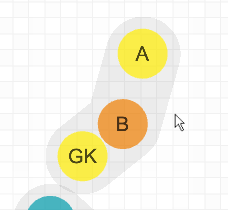
\includegraphics[width=0.3\textwidth]{pixijs-canvas-3}
    \caption{StudyMap: Supergruppe ohne Label - Hitarea}
    \bildquelle{Eigene Darstellung}
    \label{fig:pixijs-canvas-3}
\end{figure}

Schließlich besitzt jede Bubble einen zusätzlichen \code{.onmouseover()}-Eventlistener. Wenn dieses Event ausgelöst wird, wird die Bubble vergrößert und immer gegenüber eventuell überschneidenden Bubbles in den Vordergrund gestellt. Die Labels der anderen Studiengänge in allen anderen Supergruppen werden deaktiviert, um den Fokus auf diese Inhaltskategorie und explizit diese Bubble zu legen. Daraufhin erscheint darüber das Tooltip, das in \autoref{fig:pixijs-tooltip-1} zu sehen ist.

Da ein Smartphone in der Regel keine Maus angeschlossen hat, wird anstelle des für Desktop-Benutzer verwendete \code{.onmouseover()}-Event das \code{.ontap()}-Event verwendet. Dieses Ereignis wird ausgelöst, wenn der Benutzer auf die Bubble des Studiengangs tippt. Die Hitarea des Supergruppen-Nebels wird dabei ignoriert.

Auch hier muss erneut differenziert werden. Wenn ein Desktop-Nutzer auf eine Bubble klickt, öffnet sich der Dialog mit den Studiengangsdetails gemäß dem Konzept. Wenn ein Smartphone-Nutzer auf die Bubble tippt, sollte sich das Popup nicht direkt öffnen. Es ist wichtig, dass der Nutzer zuvor das Tooltip gesehen hat, um zu wissen, welchen Studiengang er öffnet.

Aus diesem Grund wird beim \code{.ontap()}-Event auf eine Bubble zwischen drei Zuständen unterschieden:

\begin{enumerate}
    \item \textbf{Bisher noch nichts anderes angetippt:} Dann wird der gleiche Hover-Effekt ausgeführt, den auch ein Desktop-Endgerät beim \code{.onmouseover()}-Event über eine Bubble auslösen würde.
    \item \textbf{Es wurde bereits eine andere Bubble angeklickt:} In diesem Fall wird der Hover-Effekt für die bereits angeklickte Bubble deaktiviert und für diese Bubble aktiviert.
    \item \textbf{Diese Bubble wurde bereits angeklickt:} Daraufhin wird das Tooltip entfernt und das Popup mit den Details zum Studiengang geöffnet. Dies ist das Äquivalent zu einem Doppelklick auf die Bubble.
\end{enumerate}

Zur Implementierung dieser Funktionalität ist die Zwischenspeicherung eines Active-State erforderlich, der immer die zuletzt angeklickte Bubble enthält.

\paragraph*{Herausforderung 2: Was passiert, wenn das Tooltip außerhalb des Bildschirms gezeichnet wird?}
Die Zeichenoberfläche von PixiJS enthält keine vorgefertigten Anzeigeelemente oder Komponenten zur Erstellung einer Benutzeroberfläche. Das bedeutet, dass Elemente wie z.B. das Tooltip in Abbildung X selbst mit Hilfe von Polygonen gezeichnet werden müssen.

Das gezeigte Tooltip besteht aus einem abgerundeten Rechteck, das den Text darüber enthält, und einem Dreieck, das anzeigt, für welche Bubble das Tooltip geöffnet wurde. Das Rechteck und das dazugehörige Dreieck werden in Schwarz aneinander gesetzt, so dass das kleine Fenster wie eine Sprechblase aussieht.

Bei der Entwicklung der Klasse Tooltip wurde festgelegt, dass die Standardrichtung zum Öffnen des Tooltips nach oben zeigt. Der folgende Codeausschnitt zeigt, wie die Richtung festgelegt wird:

\begin{lstlisting}[style=Python]
this.direction = 'top';
if (this.rootObjectYPosition - this.distance - this.container.height < 0) {
    // if object is too high to display the tooltip, it will be drawn to the bottom
    this.direction = 'bottom';
} else if (this.rootObjectXPosition - this.container.width / 2 < 0) {
    // if object overlaps left world border, it will be drawn to the right        
    this.direction = 'right';
} else if (this.rootObjectXPosition + this.container.width / 2 > this.worldWidth) {
    // if object overlaps right world border, it will be drawn to the left
    this.direction = 'left';
}
\end{lstlisting}

Die Variablen \code{this.rootObjectXPosition} und \code{this.rootObjectYPosition} enthalten die x- und y-Koordinaten des Elements, an dem der Tooltip erscheinen soll. In diesem Fall sind dies die Koordinaten der jeweiligen Bubble. Die Variable \code{this.distance} enthält den vordefinierten Abstand, um den der Tooltip vom Element entfernt sein soll. Im vorliegendem Fall handelt es sich mindestens um den Radius des Studiengangskreises. Die Größe des Tooltips wird wiederum in den Variablen \code{this.container.height} und \code{this.container.width} gespeichert.

Die Richtung des Tooltip-Fensters wird nach dem Ausschlussverfahren festgelegt. Wenn das Tooltip mit der Standardrichtung \code{'top'} (nach oben) aus der Zeichenfläche hinausragt, wird die Richtung nach unten (\code{'bottom'}) festgelegt. Anschließend wird überprüft, ob das Element die linke Fenstergrenze überschreitet. Falls dies der Fall ist, wird die Richtung auf \code{'rechts'} gesetzt. In diesem Fall wird die Richtung auf \code{'links'} gesetzt. Analog dazu wird geprüft, ob das Objekt die rechte Grenze überschreitet.

Sobald die Ausrichtung des Tooltips festgelegt wurde, müssen die Elemente einzeln verschoben und gedreht werden. Führt die vorangegangene if-Bedingung dazu, dass die Richtungsvariable \code{direction} auf \code{'left'} gesetzt wird, muss das Tooltip wie in der folgenden \autoref{fig:pixijs-tooltip-2} dargestellt links neben der Bubble erscheinen.

\begin{figure}[H]
    \centering
    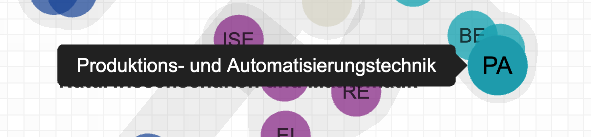
\includegraphics[width=0.6\textwidth]{pixijs-tooltip-2}
    \caption{StudyMap: Tooltip links neben Bubble}
    \bildquelle{Eigene Darstellung}
    \label{fig:pixijs-tooltip-2}
\end{figure}

Der unten dargestellte Codeauszug zeigt die Platzierung des Tooltip-Containers auf der linken Seite. Zunächst wird die Rotation des Dreiecks geändert, sodass es sich um 90 Grad nach links dreht. Anschließend werden die x- und y-Koordinaten des Dreiecks so angepasst, dass es an der rechten Seite des abgerundeten Rechtecks anliegt. Schließlich wird der gesamte Container mithilfe der Zeilen sechs und sieben linksbündig und gleichzeitig vertikal zentriert neben der Bubble platziert. Sowohl das Dreieck als auch das abgerundete Rechteck und der Text sind im Container enthalten.

\noindent
Platzierung des Tooltips auf der linken Seite:
\begin{lstlisting}[style=Python]
if (this.direction == 'left') {
    triangle.rotation = -Math.PI / 2;
    triangle.y = this.container.height / 2 - triangleHeight / 2;
    triangle.x = this.container.width;

    this.container.x = -this.container.width - this.distance;
    this.container.y = -background.height / 2;
}
\end{lstlisting}

Dieser Ansatz funktioniert jedoch nur bis zu einem gewissen Grad. Wenn das Tooltip breiter ist als die x-Achse des Endgeräts, wird es immer über die Seiten des Endgeräts hinausragen, da auf keiner der beiden Seiten genügend Platz für das Tooltip zur Verfügung steht. % TODO: In Zukunftsaussichten aufnehmen

\newpage
\subsubsection{Python - Berechnung der Positionen}
Die Berechnung der Positionen für die Studiengänge basiert, wie im Abschnitt
\ref{sec:MDS} erläutert, auf dem Multidimensionalen Skalierungsalgorithmus
(MDS), der in Python implementiert ist. Der Algorithmus verarbeitet eine
strukturierte CSV-Datei, die alle relevanten Informationen zu den Studiengängen,
Feldern und Meta-Informationen (wie z.B. Fakultätszugehörigkeit) enthält. Dieser
Datensatz bildet die Grundlage für die Positionsbestimmung im zweidimensionalen
Raum.

Hierzu wird ein Python-Skript entwickelt, welches die CSV-Datei einliest und
schließlich den MDS-Algorithmus auf den Daten anwendet. Im Verlauf der
Arbeit wurde eine anfängliche Eigenimplementierung des MDS-Algorithmus in
Betracht gezogen.

\noindent
Zu diesem Zweck wurde eine Python-Klasse erstellt, die drei Methoden enthält:
\begin{enumerate}
    \item calculate\_distance\_matrix(X)
    \item read\_data\_from\_csv()
    \item mds(self)
\end{enumerate}

Die Methode \code{calculate\_distance\_matrix} berechnet die Distanzmatrix,
welche für den Ablauf des Programms essenziell ist. Der Code dazu wird an
dieser Stelle ausgespart, da er bereits in Abschnitt \ref{sec:distanzmatrix}
vollständig spezifiziert wurde. Außerdem ausgespart ist die Methode
\code{read\_data\_from\_csv()}, welche die Eingabedatei einliest, analysiert und
schließlich die zur Berechnung benötigten Zahlen-Arrays zurückgibt. Für die Berechnung der mathematischen Gleichungen wird die Programmbibliothek NumPy verwendet. \parencite{team_numpy_2023}

\noindent
\begin{minipage}{\linewidth}
Folgender Ausschnitt eines Quellcodes beinhaltet die für diese
Arbeit entwickelte Eigenimplementierung des MDS-Algorithmus, basierend auf dem im Abschnitt
\ref{sec:MDS} genau erläuterten Ablauf:
\begin{lstlisting}[style=Python]
def mds(self):
    # Reads data from CSV file and transforms it to number rows
    X = self.read_data_from_csv()

    # Calculates distance matrix
    M = self.calculate_distance_matrix(X)

    # Double centered matrix
    n = 11 # Number of subjects
    I = np.identity(n) # Identity matrix
    Jn = np.ones((n, n)) # Matrix Jn of all ones
    C = I - (1/n) * Jn # Calculate centering matrix C
    B = -0.5 * np.dot(np.dot(C, np.array(M)), C) # Calculate the double centered matrix B

    # Eigenvalues, Eigenvectors
    m = 2  # number of dimensions (2D)
    eigenvalues, eigenvectors = np.linalg.eig(B) # Perform eigenvalue decomposition

    # Sort eigenvalues and corresponding eigenvectors in descending order
    sorted_indices = np.argsort(eigenvalues)[::-1]
    eigenvalues = eigenvalues[sorted_indices]
    eigenvectors = eigenvectors[:, sorted_indices]

    # Select the top m eigenvalues and corresponding eigenvectors
    top_m_eigenvalues = eigenvalues[:m]
    top_m_eigenvectors = eigenvectors[:, :m]

    # Calculate the square root of the diagonal matrix
    sqrt_Lambda_m = np.sqrt(np.diag(top_m_eigenvalues))

    # Compute the matrix X using the formula
    X_transformed = np.dot(top_m_eigenvectors, sqrt_Lambda_m)

    return X_transformed
\end{lstlisting}
\end{minipage}

Die Entwicklung und Umsetzung dieser eigenen Lösung erwies
sich jedoch als äußerst anspruchsvoll, da sie zahlreiche subtile mathematische
Nuancen berücksichtigen müsste. Angesichts dieser Komplexität wurde die
Entscheidung getroffen, auf die bewährte und leistungsstarke
SciKit-Learn-Bibliothek zurückzugreifen. Die Verwendung dieser etablierten
Implementierung ermöglicht eine präzise und effiziente Lösung, wobei der Fokus
auf den zentralen Fragestellungen der Masterarbeit liegt. Außerdem gewährleistet
die Einbindung von SciKit-Learn neben der Robustheit der MDS-Umsetzung, auch die
Reduktion der Entwicklungskomplexität im Hinblick auf die
Algorithmusimplementierung. \parencite{developers_scikit-learn_2023}

Das Ergebnis des Skripts sind Koordinaten für jeden Studiengang im
zweidimensionalen Raum. Diese Koordinaten werden anschließend zusammen mit den
vorher eingelesenen Meta-Daten zu den Studiengängen in JSON-Dateien gespeichert,
die schließlich vom Backend über eine Webschnittstelle bereitgestellt werden.

Der Vorteil bei der Speicherung der berechneten Positionen in Form von
JSON-Dateien liegt darin, dass die Daten wesentlich seltener geändert werden,
als die Website aufgerufen wird. Somit wird effektiv Rechenleistung und Strom
gespart. Gleichzeitig erhöht
dieses Vorgehen die Performance der Website. Zur Festigung dieser These werden
die Google Suchtrends von 2021 zum Suchbegriff \glqq OTH Regensburg
Studiengänge\grqq{} herangezogen (siehe Anhang
\ref{appendix:google-search-trends}). Die Trends zeigen eine Jahressumme von
1194 Suchanfragen. Die Anzahl an Suchanfragen lassen sich nicht 1:1 in
Seitenaufrufe projizieren, verdeutlichen aber dennoch einen ungefähren
Richtwert. Die Datengenerierung hingegen wird nach mündlicher Zusage von
Frau Rösel (Vizepräsidentin der OTH-Regensburg) nur bei größeren Änderungen an den
Inhalten von Studiengängen, oder beim Hinzufügen bzw. Entfernen eines 
Studiengangs ausgelöst. Dies wiederum passiere meist insgesamt nur einmal pro
Jahr.

Das Python-Skript hat neben der Berechnung und Speicherung der Koordinaten der Studiengänge noch eine weitere Aufgabe. Sobald der Benutzer auf der StudyMap eine Bubble anklickt, öffnet sich ein Popup mit Details zum entsprechenden Studiengang (siehe Konzept \autoref{fig:mockup-bubbles-popup}). Wie im weiteren Verlauf der Arbeit noch erläutert wird, können diese Details über die Administrationsoberfläche bearbeitet werden. Es ist jedoch notwendig, dass die Dateien mit diesen Informationen bereits angelegt werden und sowohl die Werte der Inhaltskategorien für die Darstellung mit den Balken als auch die ähnlichen Studiengänge bereits in diese Dateien geschrieben werden. Diese Funktion übernimmt das Python-Skript.

Bei der Berechnung neuer Koordinaten wird für jeden eingelesenen Studiengang eine .json-Datei mit einem leeren Template erstellt. Wenn bereits eine Datei für den Studiengang aus einer vorherigen Datenquelle existiert, wird diese geöffnet und bearbeitet. Zur späteren Darstellung der Inhaltskategorien werden anschließend die Originalwerte aus der Datenquelle in die .json-Datei kopiert (siehe folgendes Beispiel-JSON-Objekt \code{contents}).

Um ähnliche Studiengänge zu ermitteln, wird für jeden Studiengang anhand der zuvor berechneten Koordinaten der euklidische Abstand zu allen anderen Studiengängen ermittelt. Alle Studiengänge, die innerhalb einer bestimmten Grenze liegen, werden in eine Liste aufgenommen und schließlich in die .json-Datei des jeweiligen Studiengangs geschrieben (siehe folgendes Beispiel-JSON-Objekt \code{related\_studies}).

\noindent
Beispiel: Leeres Template des Studiengangs Architektur mit Inhalten und ähnlichen Studiengängen:
\begin{lstlisting}[style=Python]
{
    "name": "Architektur",
    "abb": "A",
    "supergroup": "",
    "length": 0,
    "course_url": "",
    "starting_salary": "",
    "description": "",
    "local_companies": [],
    "related_studies": [
        { "name": "Bauklimatik", "abb": "GK" },
        { "name": "Bauingenieurwesen", "abb": "B" }
    ],
    "contents": [
        { "name": "Architektur", "score": 0.43 },
        { "name": "Bau", "score": 0.25 },
        { "name": "Design", "score": 0.09 },
        { "name": "Digitalität", "score": 0.06 },
        { "name": "Elektrotechnik", "score": 0.06 },
        { "name": "Erneuerbare Energien", "score": 0.0 },
        { "name": "Future Skills", "score": 0.03 },
        ...
    ]
}
\end{lstlisting}

Falls sich im Ordner weitere .json-Dateien befinden, die von Studiengängen stammen, die in der aktuellen Datenquelle nicht mehr aufgeführt sind, werden diese automatisch gelöscht.

\newpage
\subsubsection{Node.js - REST-API}\label{sec:node-js-restapi}
Wie im vorherigen Abschnitt erläutert, ist neben dem Python-Programm auch eine Webschnittstelle erforderlich. In diesem Fall wird hierfür Node.js in Kombination mit der Bibliothek Express verwendet. Node.js ist eine JavaScript-Runtime-Umgebung, die auf der V8 JavaScript Engine von Google basiert und eine serverseitige Ausführung von JavaScript ermöglicht. \parencite{foundation_nodejs_2023} Express wiederum ist ein quelloffenes Webanwendungs-Framework für Node.js. Es erleichtert die Erstellung von Webanwendungen und APIs, indem es eine Reihe von Funktionen und Tools für den Aufbau von Webanwendungen bereitstellt.
\parencite{foundation_express_2023}

Der daraus entstehende Webservice ermöglicht den Zugriff, auf die vom Python-Skript generierten Dateien, über standardisierte REST-Endpunkte.

Eine REST-API (Representational State Transfer Application Programming Interface) ist eine zustandslose Schnittstelle, die es ermöglicht, über HTTP-Methoden, wie GET, POST oder PATCH, auf Ressourcen des Systems zuzugreifen und mit ihnen zu interagieren.

\noindent
In der folgenden \autoref{table:rest-api} werden die REST-Endpunkte von StudyMap vorgestellt. Alle Einträge mit einem \code{x} in der Spalte \textbf{Auth.} setzen eine Authentifizierung, welche im späteren \autoref{paragraph:angular-basic-auth} näher erläutert wird, voraus:
\begin{table}[!ht]
    \centering
    \begin{tabular}{|l|l|l|c|}
    \hline
    \textbf{Methode} & \textbf{Pfad}                & \textbf{Rückgabewert} & \multicolumn{1}{l|}{\textbf{Auth.}} \\ \hline
    \textbf{GET}     & /bubbles/bachelor?mode=:mode & application/json      &                                     \\ \hline
    \textbf{GET}     & /details/:abb?mode=:mode     & application/json      &                                     \\ \hline
    \textbf{GET}     & /data/history                & application/json      & x                                   \\ \hline
    \textbf{PATCH}   & /data/history/restore/:id    & application/json      & x                                   \\ \hline
    \textbf{GET}     & /data/generate?mode=:mode    & application/json      & x                                   \\ \hline
    \textbf{GET}     & /data/download/:version      & application/zip       & x                                   \\ \hline
    \textbf{POST}    & /data/upload                 & application/json      & x                                   \\ \hline
    \textbf{GET}     & /data/details                & application/json      & x                                   \\ \hline
    \textbf{PATCH}   & /data/details/:filename      & application/json      & x                                   \\ \hline
    \end{tabular}

    \caption{StudyMap-API: REST-Endpunkte}
    \label{table:rest-api}
\end{table}

Bestimmte Endpunkte enthalten so genannte Query-Parameter. Query-Parameter sind Key-Value-Paare, die an das Ende einer URL angehängt werden können, um dem Webserver zusätzliche Informationen mitzuteilen. \parencite{branch_query_2024} \autoref{table:rest-api} zeigt einige Endpunkte mit dem Query-Parameter \code{mode}.


\noindent
\begin{minipage}{\linewidth}
Beispiel für eine Anfrage:
\begin{lstlisting}[style=Python, mathescape=true]
    GET /bubbles/bachelor$\textbf{?mode=staging}$ HTTP/1.1
    Host: ...
\end{lstlisting}
\end{minipage}

\noindent
Beschreibung der in \autoref{table:rest-api} aufgezählten Endpunkte:

\paragraph*{GET /bubbles/bachelor?mode=:mode}
\vspace{-1.0em}
Gibt alle gespeicherten Bachelor-Studiengänge in einem JSON-Positions-Array aus. Darin befindet sich der Name des Studiengangs, sein Kürzel, die zugehörige Supergruppe und die Farbe der Fakultät, um die Bubble entsprechend einzufärben. Außerdem enthält jeder Studiengang die relative Position in der StudyMap, die vom Algorithmus berechnet und auf 1 normiert wurde.

\noindent
Queryparameter: \code{:mode} $\in$ {'staging', 'production'}

\noindent
\begin{minipage}{\linewidth}
Beispielausgabe:
\begin{lstlisting}[style=Python]
{
    "positions": [
        [
            "Architektur",
            "AT",
            "Architektur und Bau",
            "#A0CCCC",
            [
                0.4013795552124245,
                1.0
            ]
        ],
        ...
    ],
}
\end{lstlisting}
\end{minipage}

\paragraph*{GET /details/:abb?mode=:mode}
\vspace{-1.0em}
Sobald alle Studiengänge abgerufen wurden und der Benutzer auf eine der Bubbles klickt, öffnet sich ein Popup mit Details über den Studiengang. Der Klick ruft den Befehl \code{/details/:abb} auf, wobei \code{:abb} für das Kürzel des Studiengangs steht. Die Ausgabe ist erneut ein JSON und enthält die Details des Studiengangs.

\noindent
Queryparameter: \code{:mode} $\in$ {'staging', 'production'}

\noindent
Beispielausgabe:

\begin{lstlisting}[style=Python]
{
    "name": "Informatik",
    "abb": "IN",
    "supergroup": "Bachelor of Science (B.Sc.)",
    "length": 7,
    "course_url": "https://www.oth-regensburg.de/studieren/...",
    "starting_salary": "Überdurchschnittlich",
    "description": "Sie möchten mit Informatik die Zukunft gestalten? Informatik ist in allen Branchen ...",
    "local_companies": [
        { "name": "Vector", "url": "https://www.vector.com/" },
        ...
    ],
    "related_studies": [
        { "name": "International Computer Science", "abb": "ICS" },
        ...
    ],
    "contents": [
        { "name": "Architektur", "score": 0.0 },
        { "name": "Bau", "score": 0.0 },
        { "name": "Design", "score": 0.3 },
        { "name": "Gesundheit", "score": 0.0 },
        { "name": "Informatik", "score": 1.0 },
        { "name": "Internationales", "score": 0.2 },
        ...
    ]
}
\end{lstlisting}

\paragraph*{GET /admin/data/history}
\vspace{-1.0em}
Gibt alle existierenden (maximal zehn) Datensicherungen in einem Array aus IDs aus.

\noindent
\begin{minipage}{\linewidth}
Beispielausgabe:
\begin{lstlisting}[style=Python]
    ["1708014679710","1708014600777"]
\end{lstlisting}
\end{minipage}

\paragraph*{PATCH /admin/data/history/restore/:id}
\vspace{-1.0em}
Stellt Datensicherung mit der ID :id wieder in die Staging-Umgebung her. :id ist ein Pfadparameter.

\noindent
Beispielausgabe bei erfolgreicher Wiederherstellung (HTTP-Statuscode 200):
\begin{lstlisting}[style=Python]
{
    "message": "Starte Bearbeitung: staging -> staging\nBubbles wurden neu generiert.\nFolgende .JSON-Vorlagen wurden nicht gefunden: B, ID, HK, PA, IE, LP, SA, IW, EB, ISE, UI, MS, IR, REE, EI, ME, BE, MB, PT, ICS\nEs wurden insgesamt 4 Studiengangsvorlagen bearbeitet.\nProzess erfolgreich beendet.\n"
}
\end{lstlisting}

\noindent
Beispielausgabe bei Fehlerfall (HTTP-Statuscode 500):
\begin{lstlisting}[style=Python]
{
    "message": "Fehler beim Wiederherstellen des letzten Standes."
}
\end{lstlisting}

\paragraph*{GET /admin/data/generate?mode=:mode}
\vspace{-1.0em}
Erstellt anhand der bereits hochgeladenen Dateien eine neue Version und erzeugt im Falle einer Produktivversion eine Datensicherung.

\noindent
Queryparameter: \code{:mode} $\in$ {'staging', 'production'}

\noindent
\begin{minipage}{\linewidth}
Beispielausgabe bei Generierung einer Produktivversion (HTTP-Statuscode 200):
\begin{lstlisting}[style=Python, mathescape=true]
{
    "message": "Starte Bearbeitung: $\textbf{staging -> production}$\nBubbles wurden neu generiert.\nFolgende .JSON-Vorlagen wurden nicht gefunden: B, ID, HK, PA, IE, LP, SA, IW, EB, ISE, UI, MS, IR, REE, EI, ME, BE, MB, PT, ICS\nEs wurden insgesamt 4 Studiengangsvorlagen bearbeitet.\nProzess erfolgreich beendet.\n"
}
\end{lstlisting}
\end{minipage}

\noindent
Beispielausgabe bei Fehlerfall beim Upload von neuen Daten (HTTP-Statuscode 400):
\begin{lstlisting}[style=Python]
{
    "message": "    self.dataset = Dataset(input_path)\n  File '.../backend/generator/dataset.py', line 20, in __init__\n    for i, row in enumerate(csvreader):\n  File '.../lib/python3.9/codecs.py', line 322, in decode\n    (result, consumed) = self._buffer_decode(data, self.errors, final)\nUnicodeDecodeError: 'utf-8' codec can't decode byte 0x9f in position 14: invalid start byte\n"
}
\end{lstlisting}

\paragraph*{GET /admin/data/download/:version}
\vspace{-1.0em}
Erstellt aus der Version :version eine .zip-Datei und erstellt daraus einen Download-Stream. Für den Pfadparameter :version gilt :version $\in$ {'staging', 'production', 'template'}.

\paragraph*{POST /admin/data/upload}
\vspace{-1.0em}
Nimmt mehrere Dateien entgegen und speichert diese im Input des StudyMap-Algorithmus. Die zu hochladenden Dateien müssen im Body der HTTP-Anfrage enthalten sein. Dabei gibt es die Regeln: dataset (1 Datei), faculties (1 Datei) und details (maximal 50 Dateien). Die hochgeladenen Dateien können anschließend per Aufruf von \code{/admin/data/generate} verarbeitet werden.

\noindent
Beispielausgabe bei erfolgreichem Upload (HTTP-Statuscode 200):
\begin{lstlisting}[style=Python]
{
    "message": "Dateien erfolgreich hochgeladen."
}
\end{lstlisting}

\noindent
Beispielausgabe bei fehlerhaften Download (HTTP-Statuscode 500):
\begin{lstlisting}[style=Python]
{
    "message": "Fehler beim Dateiupload."
}
\end{lstlisting}

Durch die in diesem Unterkapitel beschriebene Web-Schnittstelle kann das PixiJS-Frontend in Echtzeit die benötigten Informationen abrufen, um die interaktive Grafik der Studiengänge zu erstellen. Die klare Trennung von Backend und Frontend gewährleistet eine effiziente Datenübertragung und ermöglicht eine dynamische Aktualisierung der Grafik bei Änderungen im Datensatz.

\paragraph*{GET /admin/data/details}
\vspace{-1.0em}
Dieser Endpunkt ruft die Dateinamen aller gespeicherten Studiengangsdetails ab und gibt sie aus. Wenn die Inhalte per .csv-Datei hochgeladen werden, wird für jeden Studiengang, sofern noch nicht vorhanden, eine .json-Datei mit den Studiengangsdetails erstellt. Mithilfe dieses Endpunkts können die Dateinamen dieser Dateien abgerufen werden.

\noindent
Beispielausgabe nach erfolgtem Upload von Studiengängen (HTTP-Statuscode 200):
\begin{lstlisting}[style=Python]
[
    "A.json","B.json","BE.json","BM.json","DBM.json","EI.json","GK.json",
    "I.json","IBM.json","ICS.json","ID.json","IR.json","ISE.json","IT.json",
    "IW.json","KI.json","MB.json","ME.json","MS.json","PA.json","RE.json",
    "SC.json","UI.json"
]
\end{lstlisting}

\paragraph*{PATCH /admin/data/details/:filename}
\vspace{-1.0em}
Nachdem alle verfügbaren Studiengänge mit /admin/data/details abgerufen wurden, können mithilfe von \code{/details/:abb} die Details zu einem einzelnen Studiengang abgefragt werden. Anschließend kann der Benutzer die Informationen in der Administrationsoberfläche bearbeiten und die Änderungen mit diesem Endpunkt der API persistieren.

Der Request Body dieser Anfrage muss das bearbeitete JSON-Objekt der Studiengangsdetails sein. Der Request Body enthält die zu sendenden Daten der HTTP-Anfrage. \parencite{parthiban_essential_2023}

Bei erfolgreicher Speicherung der Studiengangsdetails wird zusammen mit dem Statuscode 200 der neue Inhalt der Datei zurückgegeben. Ein Beispiel dazu befindet sich in der Schnittstellenbeschreibung für \code{GET /details/:abb}.

\noindent
Wenn der Prozess fehlschlägt, gibt es zwei Arten von Fehlermeldungen zu unterscheiden:
\begin{itemize}
    \item \textbf{Der Speicherprozess ist fehlgeschlagen:} In diesem Fall wird der Statuscode 500 zusammen mit der Fehlerbeschreibung als JSON ausgegeben: \lstinline[style=python]|{"message": "Fehler bei der Aktualisierung der Studiengangsdetails."}|.
    \item \textbf{Die angeforderte Datei \code{:filename} existiert nicht:} Der Statuscode 404 wird mit dem JSON \lstinline[style=python]|{"message": "Studiengangsdetails nicht gefunden."}| zurückgegeben. 
\end{itemize}

\subsubsection{Angular - Administrationsoberfläche}
Um den im \autoref{sec:verwaltungssoftware} aufgeführten Anforderungen wie Datensicherung und Trennung von Staging- und Produktivumgebung gerecht zu werden, ist die Implementierung einer Verwaltungssoftware notwendig. Um die Entwicklung möglichst zukunftssicher, d.h. leicht erweiterbar zu gestalten, wird ein sogenanntes Webframework eingesetzt.

Ein Webframework ist eine Sammlung von Bibliotheken, Tools und Technologien und bietet Programmierern ein Grundgerüst für eine dynamische Webanwendung. Neben der Zeitersparnis durch die bereits vorhandenen Bausteine hat die Verwendung eines Webframeworks den Vorteil, dass es in der Regel eine standardisierte Struktur vorgibt, die es späteren Entwicklern erleichtert, an dem Projekt weiterzuarbeiten. Generell arbeiten die meisten Frameworks nach dem DRY-Prinzip (Don't repeat yourself), was den Code schlanker und damit weniger fehleranfällig macht.
\parencite{domainfactory_beliebtesten_2023}

Für die Entwicklung der Administrationsoberfläche wurde Angular als Webframework gewählt. Der Grund für die Wahl des Frameworks liegt in seiner Verbreitung, da Angular neben dem React-Framework und Vue.js eines der meistgenutzten Frontend-Frameworks ist. \parencite{greif_state_2022}

Angular ist ein komponentenbasiertes Framework zur Erstellung von skalierbaren Webanwendungen auf Basis der Programmiersprache TypeScript. Es enthält unter anderem Bibliotheken für das Routing zwischen Seiten, dynamische Formulare, Client-Server-Kommunikation und mehr \parencite{google_inc_angular_2023}. 

Zusätzlich zum Angular-Framework wird ein CSS-Framework benötigt, um vordefinierte Styles und wiederverwendbare Komponenten wie z.B. Dialoge zu erhalten.

HTML steht für HyperText Markup Language und ist die Sprache des Internets. HTML ist eine Dokumentenbeschreibungssprache, mit der die Struktur von Webseiten definiert wird. Mithilfe von CSS wird dann das Layout und Aussehen der in HTML definierten Elemente (z.B. Schaltflächen) festgelegt. \parencite{mozilla_corporation_html_2023} CSS wiederum steht für Cascading Style Sheets und definiert Darstellungsregeln für HTML-Elemente. CSS-Regeln enthalten Definitionen zu Größe, Form, Farbe, Animation und Layout der einzelnen HTML-Elemente einer Website. \parencite{mozilla_corporation_what_2024}

Im Fall von StudyMap wird Angular Material UI verwendet. Angular Material UI ist ein von Google entwickeltes CSS-Framework. Die Entscheidung für dieses Framework beruht darauf, dass es ebenso wie das Angular Framework von Google LLC entwickelt wurde und daher sehr gut parallel kombiniert werden kann. \parencite{google_llc_angular_2024}

Die Implementierung der Authentifizierung in Angular ist vorerst nicht erforderlich, da diese bereits durch die Authentifizierungs-Middleware der Node.js-API abgedeckt ist.

\noindent
Die Verwaltungssoftware hat in ihrer ersten Version fünf Seiten:
\begin{itemize}
    \item Überblick
    \item Neue Daten einpflegen
    \item Studiengangsdetails
    \item Versionsverlauf
    \item Vorlagen
\end{itemize}

\paragraph*{Überblick}
Die Seite \glqq Überblick\grqq{} bietet einen Überblick über das Gesamtsystem. Wie in \autoref{fig:adminui-overview-1} zu sehen ist, enthält die Seite einen Link zur Vorschau der Staging-Umgebung sowie einen Link zur Vorschau der Produktivumgebung. Des Weiteren verfügt die Seite über einen roten Knopf. Bei Bestätigung wird die Staging-Version in die Produktivumgebung überführt und somit der Öffentlichkeit freigeschaltet.

\begin{figure}[H]
    \centering
    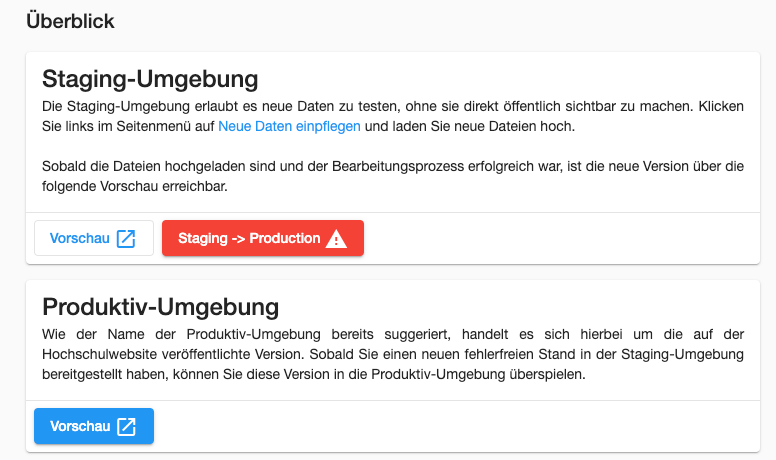
\includegraphics[width=0.8\textwidth]{adminui-overview-1}
    \caption{Admin UI: Überblick}
    \bildquelle{Eigene Darstellung}
    \label{fig:adminui-overview-1}
\end{figure}

Direkt unterhalb befinden sich auf der Übersichtsseite außerdem zwei Architekturgrafiken, die dem Benutzer die Struktur von StudyMap und die damit verbundene Datensicherung über die Versionshistorie verdeutlichen sollen.

\paragraph*{Neue Daten einpflegen}
Auf der Seite zur Eingabe neuer Daten gibt es die Möglichkeit, zwei CSV-Dateien vom Computer auszuwählen (siehe \autoref{fig:adminui-new-data-1}). Dies ist die Datenquelle, die in Kapitel X beschrieben wurde. Sie enthält alle Studiengänge und die dazugehörigen Werte der Inhaltskategorien. Die zweite Datei enthält die Abkürzungen der Fakultäten und den entsprechenden Farbcodes, um die Bubbles entsprechend den Fakultäten einzufärben.

\begin{figure}[H]
    \centering
    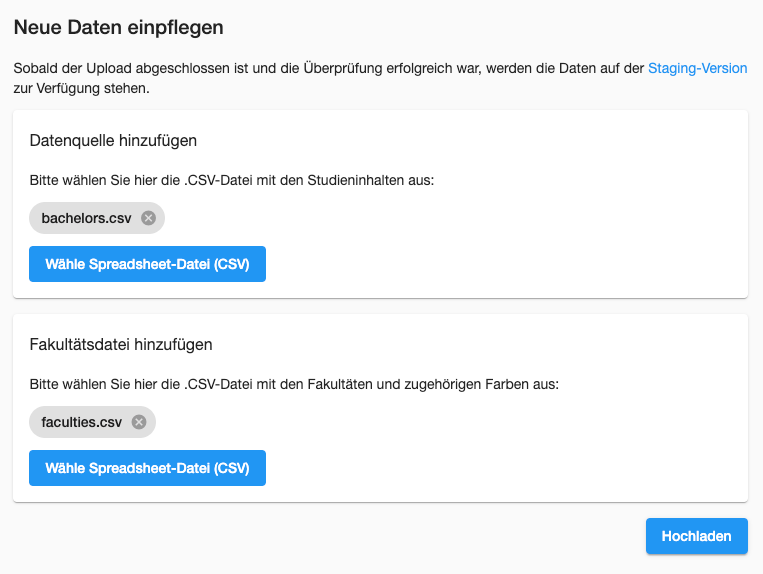
\includegraphics[width=0.8\textwidth]{adminui-new-data-1}
    \caption{Admin UI: Neue Daten einpflegen}
    \bildquelle{Eigene Darstellung}
    \label{fig:adminui-new-data-1}
\end{figure}

Nach der Auswahl der beiden Dateien können diese mithilfe der Schaltfläche \glqq Hochladen\grqq{} hochgeladen und verarbeitet werden. Sobald das Hochladen abgeschlossen ist, beginnt die Verarbeitung der Dateien. Anschließend erscheint ein Dialogfeld mit der Antwort des Servers (siehe \autoref{fig:adminui-new-data-2}).

\begin{figure}[H]
    \centering
    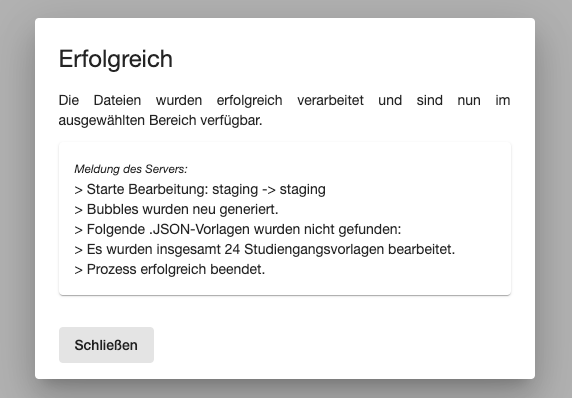
\includegraphics[width=0.5\textwidth]{adminui-new-data-2}
    \caption{Admin UI: Neue Daten einpflegen - Ergebnisdialog}
    \bildquelle{Eigene Darstellung}
    \label{fig:adminui-new-data-2}
\end{figure}

\paragraph*{Neue Daten einpflegen}
\begin{figure}[H]
    \centering
    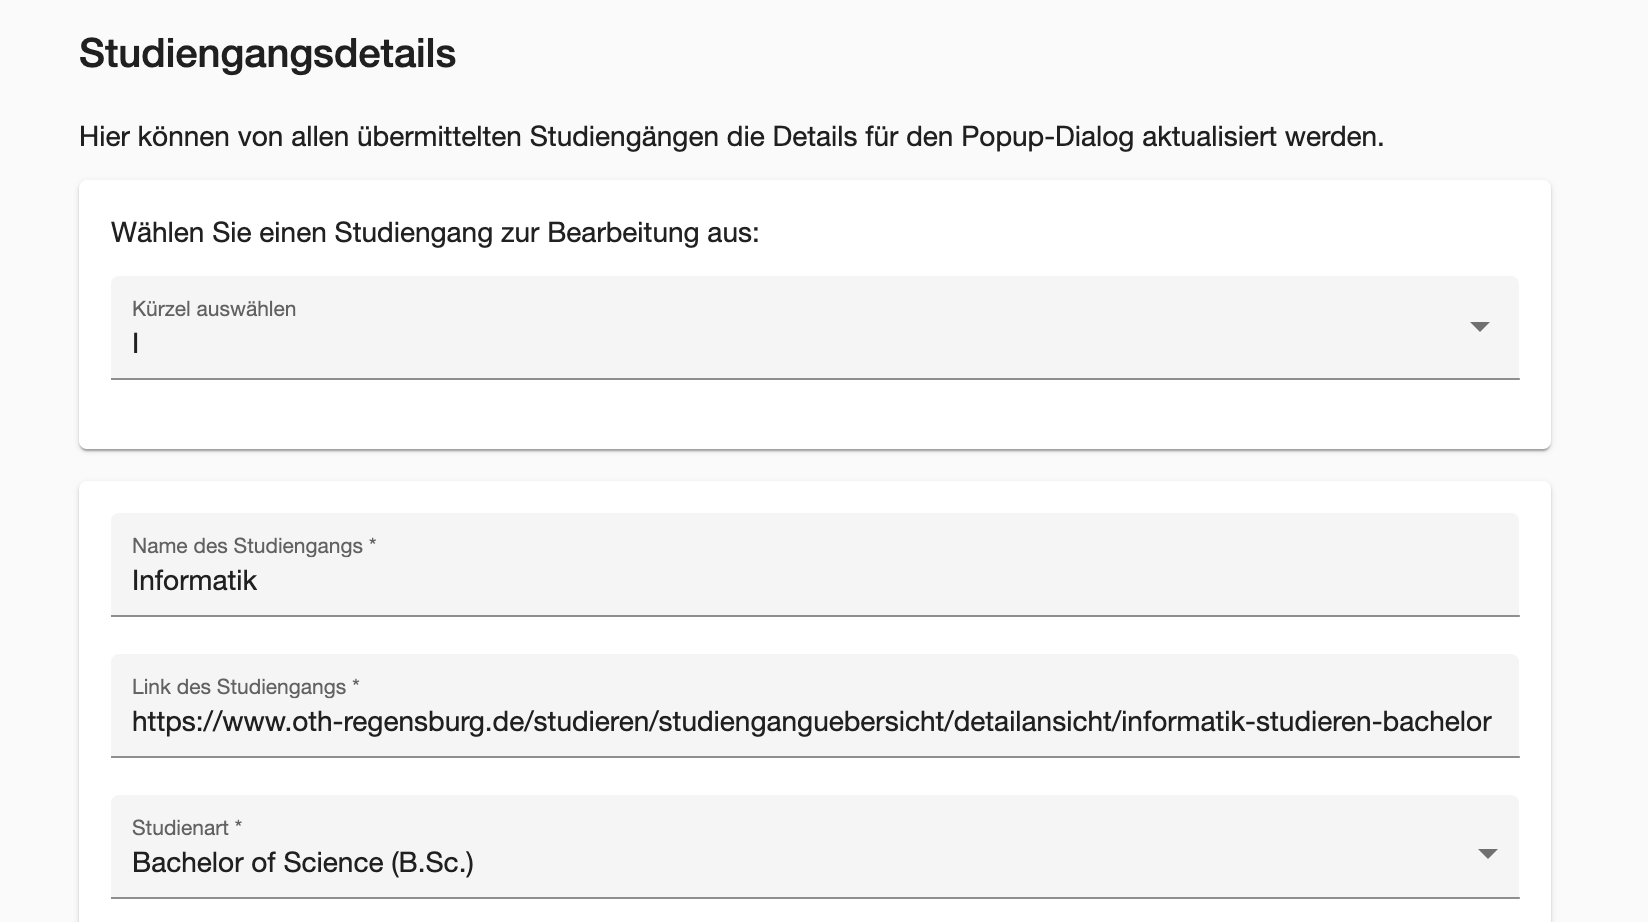
\includegraphics[width=0.8\textwidth]{adminui-details-1}
    \caption{Admin UI: Studiengangsdetails verwalten (Ausschnitt)}
    \bildquelle{Eigene Darstellung}
    \label{fig:adminui-details-1}
\end{figure}

Sobald die Dateien hochgeladen wurden, wird für jeden Studiengang eine Studiengangsdetails-Datei angelegt. Diese kann mithilfe eines grafischen Formulars in der Administrationsoberfläche bearbeitet werden. \autoref{fig:adminui-details-1} zeigt einen Ausschnitt dieses Formulars. Zunächst muss der zu bearbeitende Studiengang oben im Auswahlfenster ausgewählt werden. Anschließend können alle statischen Inhalte des Popups, das sich beim Klick auf eine Bubble in der StudyMap öffnet, bearbeitet werden. Die Liste der lokalen Unternehmen ist ebenfalls Teil davon.

% TODO: CONTINUE HERE!

\newpage
\subsection{Softwarearchitektur}
Das Gesamtbild StudyMap setzt sich aus den vorher genauer erläuterten Komponenten REST-API, PixiJS, Python-Backend und Node.js als Webserver für alle Dienste zusammen. Dieses Kapitel beschäftigt sich mit der Architektur und der Kommunikation der einzelnen Komponenten untereinander.

Obwohl die Softwarearchitektur erst in den letzten 30 Jahren an Bedeutung gewonnen hat, ist sie ein fester Bestandteil der Softwareentwicklung und definiert wesentliche tragende Säulen des Produkts. Dabei geht die Softwarearchitektur nicht auf die internen Details einer bestimmten Komponente ein. \parencite{vogel_einleitung_2009} Sie soll komplexe Zusammenhänge übersichtlich darstellen und Fragen wie folgende beantworten:
\begin{itemize}
    \item Wie hängen die Systembausteine miteinander zusammen?
    \item Welche Schnittstellen haben die Komponenten?
    \item Worauf sind Strukturierungen und Entscheidungen zurückzuführen?
\end{itemize}

Für StudyMap ist eine Darstellung der Softwarearchitektur aus mehreren Gründen essentiell.

\paragraph*{Grund 1: Komplexität}
Die Komplexität der Software wird übersichtlicher dargestellt. Da bei der Verwendung mehrerer Programmiersprachen wie JavaScript, TypeScript und Python schnell die Übersicht über die einzelnen Komponenten verloren gehen kann, besteht die Gefahr, ineffizienten oder im schlimmsten Fall fehlerhaften Code zu produzieren. Ein weiterer Grund ist die Einarbeitung zukünftiger Entwickler.

\paragraph*{Grund 2: Einarbeitung}
Da StudyMap im Rahmen dieser Masterarbeit entsteht, ist es abzusehen, dass es immer wieder wechselnde Stakeholder und Weiterentwickler für das Projekt geben wird. Diese müssen zwangsläufig eingearbeitet werden und das Gesamtprojekt verstehen. Ein Entwickler, dem der gesamte Workspace ohne Strukturgrafik mit vier miteinander kommunizierenden Projekten präsentiert wird, könnte überfordert sein. Deshalb dient die Softwarearchitektur der effizienten Einarbeitung.

\paragraph*{Grund 3: Sicherheit}
Schließlich ist die Strukturgrafik für die Sicherheit der Hochschule von Bedeutung. StudyMap enthält einen geschützten Administrationsbereich. Es sollte im Vorfeld genau festgelegt werden, dass z.B. der Administrationsbereich nur über das VPN der Hochschule erreichbar ist, um die Wahrscheinlichkeit eines Hackerangriffs zu reduzieren. Solche Beziehungen lassen sich mithilfe der Definition einer Softwarearchitektur präzise festlegen. Außerdem benötigt man diese Darstellung explizit an der OTH-Regensburg, um einen Server vom Rechenzentrum für das Hosting von StudyMap zu erhalten. Weitere Informationen dazu finden Sie im \autoref{sec:deployment}.

\begin{figure}[H]
    \centering
    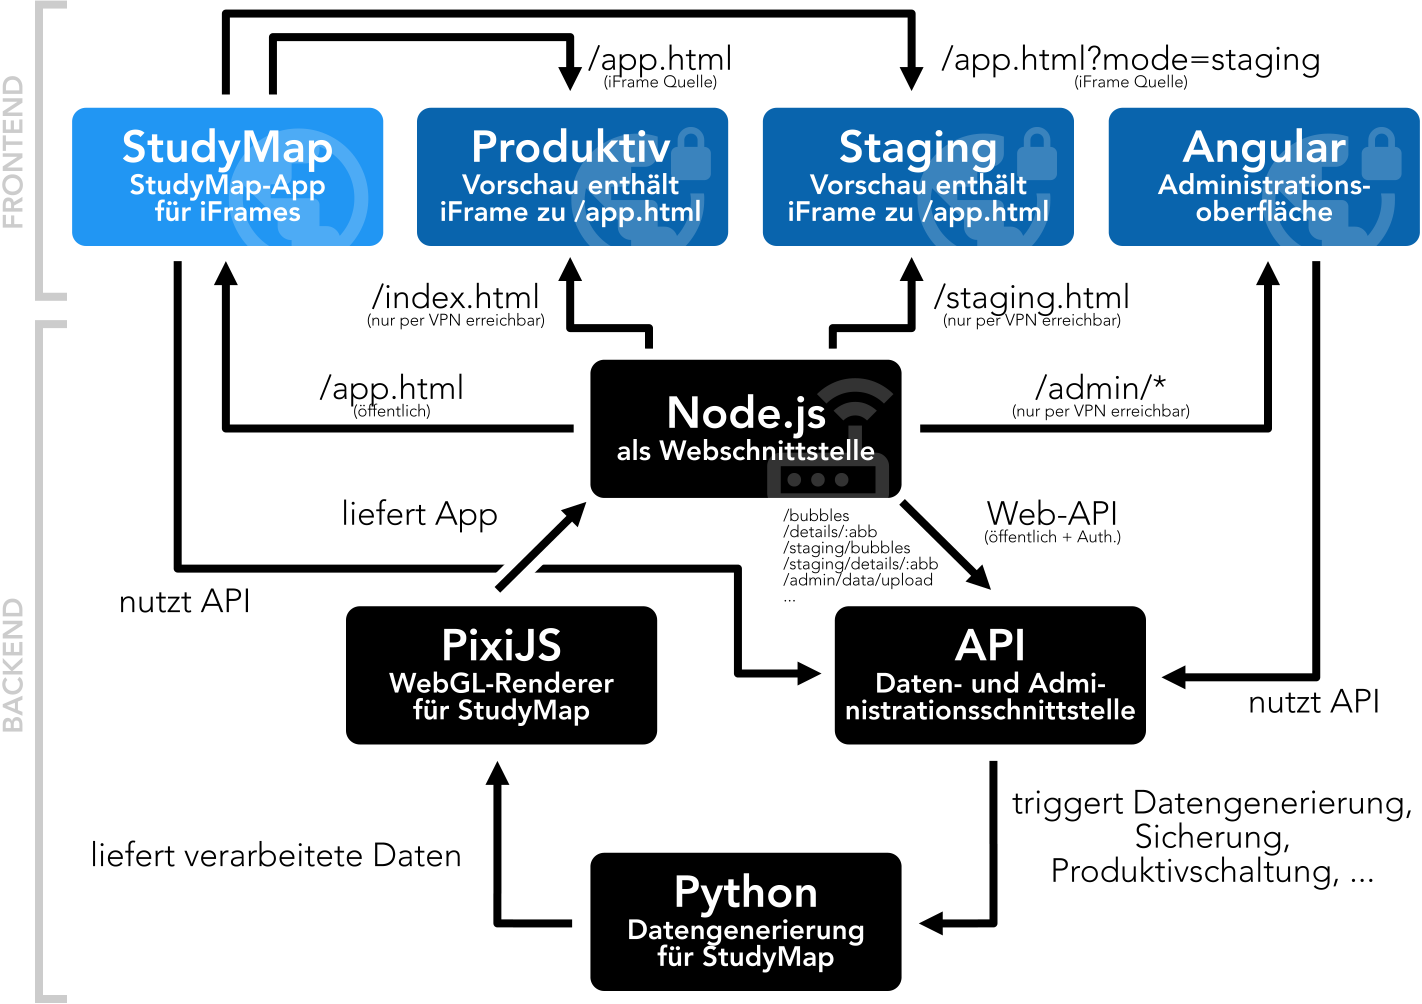
\includegraphics[width=\textwidth]{architecture}
    \caption{Softwarearchitektur von StudyMap}
    \bildquelle{Eigene Darstellung}
    \label{fig:studymap-architecture}
\end{figure}

\autoref{fig:studymap-architecture} zeigt die Softwarearchitektur von StudyMap. Die Anwendungskomponenten werden durch abgerundete Rechtecke beschrieben. Die schwarzen Rechtecke repräsentieren die Backend-Komponenten, während die blauen die Frontend-Komponenten darstellen. Die Beziehungen zwischen den Komponenten werden durch Pfeile visualisiert.

\subsubsection{Frontend-Komponenten}\label{sec:frontend-komponenten}
Alle Frontend-Komponenten werden über die Node.js-Webschnittstelle gehostet. Node.js wird mithilfe von Express genutzt, um neben der in \autoref{sec:node-js-restapi} erläuterten REST-API auch die restlichen Webseiten wie die Anwendung selbst und die Administrationsoberfläche bereitzustellen. Die Frontend-Komponenten in Dunkelblau sind ausschließlich über eine aktive VPN-Verbindung der Hochschule erreichbar.

\paragraph*{StudyMap}
Die Frontend-Komponente StudyMap ist das fertige Produkt. Die StudyMap-App besteht aus dem PixiJS-Canvas, der mit Bootstrap verbunden ist, um den Studiengangsdetails-Dialog anzuzeigen (siehe \autoref{fig:mockup-bubbles-popup}). Es handelt sich um eine reine Web-App ohne weitere Design-Elemente rund um den Canvas herum. Der Grund dafür ist, dass die StudyMap-Anwendung als iFrame in die Website der Hochschule eingebunden wird, d.h. die Anwendung muss den gesamten Bildschirminhalt ausfüllen, damit sich der iFrame später nahtlos in die Hochschulwebsite einfügt. Das HTML-Element iFrame erlaubt die Einbindung externer Webseiten in eine Seite. Ein klassisches Beispiel hierfür ist die Einbindung einer Anfahrtskarte eines Kartendienstleisters wie OpenStreetMap auf Unternehmenswebsites. \parencite{mozilla_corporation_iframe_2024} In dieser Arbeit wird der Studiengangsfinder in die Hochschulwebsite eingebettet.

\noindent
Webschnittstelle: \code{/app.html}

\paragraph*{Produktiv}
Wie in \autoref{fig:studymap-architecture} dargestellt, ist die Produktiv-Schnittstelle eine HTML-Website, die die StudyMap-App per iFrame einbettet.  Das Bestreben ist es, ein möglichst realitätsnahes Produktivsystem nachzubilden, weshalb die Produktivkomponente einen ähnlich breiten Platz für den iFrame verwendet, wie er auch auf der Website der OTH zur Verfügung steht. Die Produktivkomponente ist ausschließlich über das VPN der Hochschule erreichbar.

\noindent
Webschnittstelle: \code{/index.html}

\paragraph*{Staging}
Die Staging-Umgebung ist identisch zur Produktivumgebung. Der einzige Unterschied besteht darin, dass die StudyMap-App nicht mit \code{/app.html}, sondern mit \code{/app.html?mode=staging} eingebunden wird. StudyMap soll die Daten aus dem Staging-Bereich des Backends abrufen und darstellen.

Mit dieser Testseite können neue Daten vor der Veröffentlichung getestet und optimiert werden. Die Staging-Komponente ist ebenfalls nur per VPN erreichbar.

\noindent
Webschnittstelle: \code{/staging.html}

\paragraph*{Angular}\label{paragraph:angular-basic-auth}
Die vierte und letzte Komponente ist die Angular-Administrationsoberfläche. Offensichtlich darf auch dieser Teil der Anwendung nur über eine authentifizierte VPN-Verbindung erreichbar sein. Der gesamte Administrationsbereich ist außerdem durch eine Basic-Auth-Middleware geschützt.

\begin{figure}[H]
    \centering
    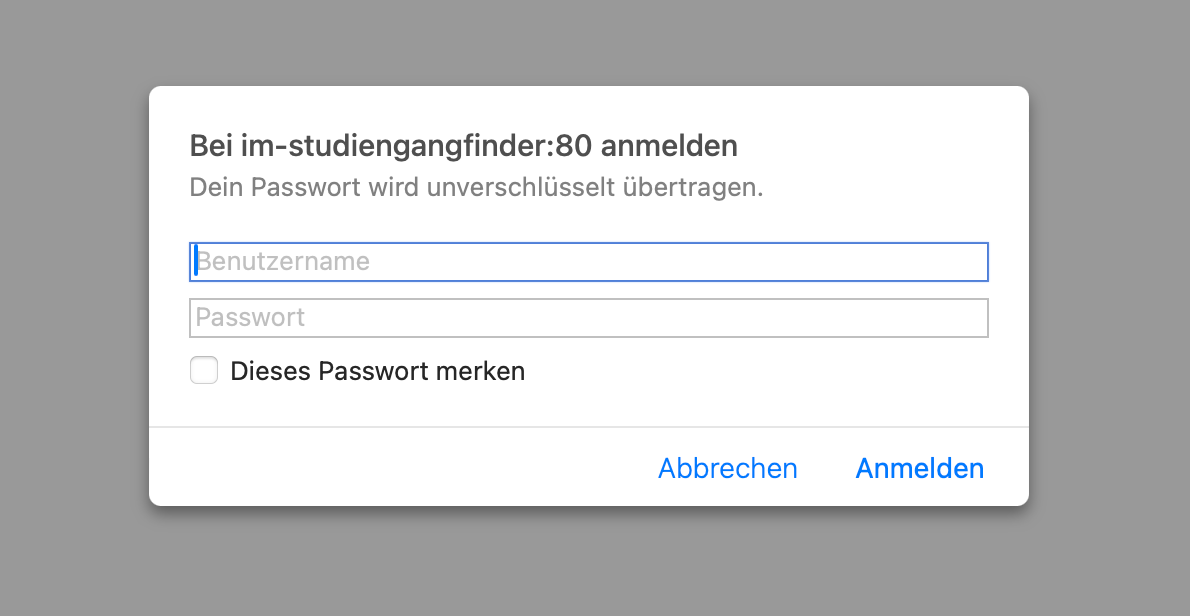
\includegraphics[width=0.6\textwidth]{basic-auth}
    \caption{Basic-Auth-Middleware von StudyMap}
    \bildquelle{Eigene Darstellung}
    \label{fig:basic-auth}
\end{figure}

Basic-Auth ist ein allgemeines Authentifizierungsframework, das standardmäßig in der HTTP-Definition enthalten ist. \parencite{mozilla_corporation_http_2023} Es wird von allen gängigen Browsern unterstützt und erfordert nicht die Implementierung eines eigenen Authentifizierungsverfahrens. \parencite{fyrd_headers_2024} Wenn ein Webserver, in diesem Fall das Node.js-Webinterface, eine Authentifizierung anfordert, können Browser diese Anforderung verarbeiten und ein generisches Anmeldeformular anzeigen (siehe \autoref{fig:basic-auth}).

In \autoref{fig:basic-auth} fehlt ein SSL-Zertifikat, wodurch keine verschlüsselte Verbindung möglich ist. SSL-Zertifikate sind kleine Datendateien, die kryptografische Schlüssel digital an eine Organisation binden. Somit können HTTPS-Verbindungen genutzt werden, welche wiederum die Browserverbindungen verschlüsseln und somit auch die eingegebenen Daten vor Mitlesern schützen. \parencite{globalsign_was_2023}

Daher wird auch eine Basic-Auth-Authentifizierung als unsicher eingestuft, wenn kein SSL-Zertifikat vorhanden ist. Um die Sicherheitsbedenken von StudyMap auszuschließen, sollte in Zukunft die Authentifizierung über einen externen Authentifizierungsprovider der Hochschule erfolgen. Dadurch muss StudyMap keine Anmeldedaten speichern und es besteht kein Risiko mehr für einen Hackangriff.

Nach Abschluss der Authentifizierung kann der Nutzer die Administrationsoberfläche nutzen. Die Web-App dient der Verwaltung der Anwendung und ihrer Daten. Hierfür werden HTTP-Anfragen genutzt, um die REST-API aufzurufen.

\noindent
Webschnittstelle: \code{/admin/*}

\subsubsection{Backend-Komponenten}
Das Backend der Softwarearchitektur besteht neben der bereits im \autoref{sec:frontend-komponenten} erläuterten Node.js Webschnittstelle aus drei weiteren Komponenten: \begin{enumerate}
    \item PixiJS: WebGL-Renderer für StudyMap
    \item API: Daten- und Administrationsschnittstelle
    \item Python: Datengenerierung für StudyMap
\end{enumerate}

\paragraph*{PixiJS}
Das PixiJS-Projekt ist ein eigenständiges JavaScript-Projekt, das die vorher erläuterte HTML-Datei \code{app.html} für die Frontend-Komponenten generiert und darin den WebGL-Renderer für StudyMap einbindet. Dieses Projekt enthält HTTP-Anfragen zur REST-API, um die Daten der Studiengänge abzurufen. Es ist jedoch wichtig zu beachten, dass diese Anfragen durch den Browser-Client bzw. die Frontend-Komponenten aufgerufen werden und somit streng genommen kein Teil der Backend-Komponente ist.

\paragraph*{API}
Die API (Application Programming Interface) bietet nicht nur die Lieferung von Positions- und Studiengangsdetailsdaten, sondern auch die Möglichkeit, die im Server gespeicherten Daten zu verwalten und zu ändern (siehe \autoref{sec:node-js-restapi}). Aus diesem Grund ist die Administrationsoberfläche sowie die StudyMap-App selbst mit der API verbunden.

Wenn jemand in der Administrationsoberfläche neue Dateien hochlädt, wird eine Anfrage an die API gesendet. Diese speichert die Dateien an der richtigen Stelle und löst schließlich die Generierung neuer Positionsdaten durch eine Anfrage an die Python-Komponente aus. Die Python-Komponente ist folglich ebenfalls mit der API angebunden.

\paragraph*{Python}
Die Python-Komponente hat im Wesentlichen nur eine wirkliche Verbindung zu einer anderen Komponente, nämlich zur REST-API, die Python aufruft. Die Python-Komponente enthält die Logik für die Generierung der auszuliefernden Dateien sowie für die Datensicherung. Das Python-Skript implementiert den MDS-Algorithmus zur Berechnung der genauen Positionsdaten anhand der Ähnlichkeiten zwischen den Studiengängen. Beide Anwendungsfälle werden durch die Kommandozeile der REST-API getriggert.

Es besteht eine weitere implizite Verbindung zwischen PixiJS und den Daten des Python-Skripts für die Anzeige der Bubbles. Die eigentliche Kommunikation zwischen den Komponenten erfolgt jedoch über die Programmierschnittstelle.

\newpage
\subsection{Software Deployment}\label{sec:deployment}
Nachdem die Softwarearchitektur geklärt und implementiert wurde, folgt in diesem Abschnitt das Deployment. Software Deployment (Softwareverteilung) bezeichnet den Prozess der Konfiguration und Installation auf dem Zielserver. Dieser Prozess besteht in der Regel aus mehreren Schritten, wie Planung, Design, Testen, Terminplanung und Deployment. \parencite{atera_team_was_2023} Im Falle von StudyMap beschränkt sich der Prozess auf die Schritte: Planung, Testen und Bereitstellung.

\subsubsection{Planung}
Der erste Schritt des Softwareverteilungs Prozesses ist die Planung, welcher diverse W-Fragen beantwortet. Es ist beispielsweise wichtig zu berücksichtigen, wie viele Nutzer die Anwendung später haben werden, welche Risiken zu erwarten sind und wie eine Authentifizierung aussehen könnte. \parencite{atera_team_was_2023}

Bei dieser Arbeit waren bereits einige Planungspunkte vorgegeben, da an der Hochschule Regensburg ein spezielles IT-Verfahren zum Schutz der Hochschule eingesetzt wird. Um das Projekt StudyMap auch nach der Übergabe der Masterarbeit weiterführen zu können, wurde eine gewisse Normbeschreibung erstellt. In der folgenden Liste sind einige ausformulierte Punkte und Details des Planungsschrittes aufgeführt.

\paragraph*{Wer sind die Verantwortlichen für die Software?}
Die Verfahrensverantwortliche Person ist Prof. Dr.-Ing. Birgit Rösel, Vizepräsidentin der OTH-Regensburg. Sie hat den Bedarf der Studienorientierung erkannt und das Projekt initiiert. Während der Entwicklung ist Andreas Huber, der Autor dieser Arbeit, die technisch verantwortliche Person.

Die technisch Verantwortliche Person ist für die Wartung und das Patchmanagement zuständig. Es ist erforderlich, alle Pakete und Programme auf dem neuesten Stand zu halten, um die Wahrscheinlichkeit eines Hackerangriffs zu minimieren. Nach Abgabe dieser Arbeit wird das Amt an eine zum Zeitpunkt des Schreibens noch unbekannte Person übertragen.

\paragraph*{Wie viele Benutzer wird die Anwendung haben?}
Diese Frage ist insbesondere für die Leistung und die benötigten Serverressourcen von Bedeutung. Zum Zeitpunkt der Entwicklung liegen keine konkreten Besucherzahlen vor. Die Softwarearchitektur ist jedoch so geplant, dass die beschriebene REST-API lediglich .json-Dateien liest und zurückgibt - dies erfordert wenig Rechen- und Netzwerkleistung. Außerdem wird die interaktive Grafik clientseitig berechnet, also auf dem Gerät des Benutzers.

Aus den genannten Gründen wird ein leistungsschwacher virtueller Server mit den folgenden Spezifikationen vom Rechenzentrum angefordert:
\begin{itemize}
    \item Prozessorkerne: 1 Kern
    \item Arbeitsspeicher: 8 GB
    \item Festplattenspeicher: 100 GB
    \item Betriebssystem: Debian 12
\end{itemize}

\paragraph*{Wie kritisch ist ein Ausfall des Systems?}
Ein Ausfall des Projekts ist weniger schwerwiegend, da es sich nur um ein optionales Feature der Hochschulwebsite handelt. Aus diesem Grund reicht es, das System innerhalb einer Wochenfrist wiederherzustellen. Darüber hinaus wird die Gesamtfunktion nicht ständig überwacht.

\paragraph*{Werden personenbezogene Daten gespeichert?}
Um rechtliche Fragen abzusichern, muss geklärt werden, ob im Falle eines Angriffs das Risiko besteht, persönliche Informationen zu verlieren. Daher ist es wichtig zu ermitteln, ob personenbezogene Daten gespeichert werden. StudyMap ist eine unabhängige Software, die Informationen über Studiengänge enthält, welche bereits veröffentlicht wurden. Das Hochladen und Speichern dieser Informationen in StudyMap durch eine verantwortliche Person ist ohne die Eingabe personenbezogener Daten möglich.

Aus diesem Grund gehören die verarbeiteten Informationen zur Hochschul-Informationsklasse \glqq V0 - öffentlich\grqq{}. Dies bedeutet, dass keine der verarbeiteten oder gespeicherten Informationen im Falle eines Diebstahls als kritisch eingestuft werden würde.

\paragraph*{Wie wird sichergestellt, dass gewisse Bereiche nur per VPN zugänglich sind?}
% TODO

\paragraph*{Wie wird die Authentifizierung sichergestellt?}
Wie bereits in \autoref{paragraph:angular-basic-auth} erläutert, wird die Authentifizierung mittels einer Middleware im Webserver sichergestellt. Zudem wird vom Rechenzentrum eine separate IP-Adresse angefordert, um den Zugriff auf bestimmte Bereiche, wie beispielsweise den Administrationsbereich, nur mit aktiver VPN-Verbindung zu ermöglichen. % TODO: Wirklich so?

\paragraph*{Welche Rollen sind vorgesehen?}
In engem Zusammenhang mit der Frage der Authentifizierung steht die Frage, welche Rollen in der Anwendung vorgesehen sind. Im Studiengangsfinder gibt es lediglich zwei Rollen:
\begin{enumerate}
    \item Administrator
    \item Besucher
\end{enumerate}
Die Besucher-Identität hat ausschließlich Zugriff auf die Frontend-Komponente \code{app.html}, welche die interaktive Grafik enthält. Eine Authentifizierung ist nicht erforderlich. Die Administrator-Identität hingegen hat Zugriff auf alle weiteren Frontend-Komponenten und kann somit die gespeicherten Daten verwalten.

\paragraph*{Wer kümmert sich um die Aktualität der Daten?}
Frau Rösel ist für die Aktualität der Daten verantwortlich, während der Entwicklung und nach der Übergabe des Projekts für einen unbestimmten Zeitraum. Nach Abgabe dieser Arbeit wird Andreas Huber, der technische Verantwortliche, Sie unverzüglich über den Prozess der Datenverwaltung durch die Administrationsoberfläche instruieren. Wer die Daten langfristig pflegt bleibt noch offen.

\paragraph*{Werden regelmäßige System- und Datensicherungen duchgeführt?}
Der Server von StudyMap befindet sich im zentralen Serverraum des Rechenzentrums der OTH-Regensburg. Dadurch wird sichergestellt, dass die Organisation täglich eine Systemsicherung durchführt.

Eine Datensicherung erfolgt nur beim Überführen eines Datenstands von Staging in die Produktivumgebung. Wie bereits beschrieben, speichert StudyMap immer die letzten 10 Produktivstände, um im Falle von korrupten Daten eine Datensicherung wiederherstellen zu können. Es gibt keine zeitgesteuerten Intervall-Datensicherungen.

\paragraph*{Was ist der Ablauf bei einem eintretenden Sicherheitsvorfall?}
Sollte es zu einer Kompromittierung des Servers kommen, muss die verantwortliche Person sofort Kontakt mit security@oth-regensburg.de aufnehmen und diese über den Vorfall informieren.

\paragraph*{Wer stellt ein SSL-Zertifikat zur verschlüsselten Übertragung der Daten?}
Damit die Verbindung zu StudyMap funktioniert, wird ein SSL-Zertifikat sowohl für die internen (VPN-Bereich) als auch für die externen Anfragen benötigt.

Wenn kein SSL-Zertifikat auf dem Webserver installiert ist, werden die Login-Anfragen unverschlüsselt verschickt. Ein Angreifer könnte dadurch die Zugangsdaten mitlesen und daraus einen weiteren Hackangriff starten.

Obwohl keine sicherheitsrelevanten Informationen beim Öffnen der Besucheransicht geteilt werden, benötigt StudyMap auch für den öffentlichen Bereich ein SSL-Zertifikat. Der Grund dafür ist, dass die Hochschulwebsite eine https-Verbindung erzwingt. Moderne Browser erlauben es nicht, einen iFrame mit einer unverschlüsselten Website auf einer verschlüsselten Website einzubinden. \parencite{vyas_mixed_2013}

\subsubsection{Testen}
In dieser Phase des Deployment-Prozesses wird eine Testumgebung erstellt, um zu überprüfen, ob alles wie vorgesehen funktioniert. Ziel ist die Schaffung einer möglichst realitätsnahen Umgebung, damit der endgültige Prozess der Bereitstellung auf dem Server der Universität mit möglichst wenigen unvorhersehbaren Komplikationen verbunden ist.

\paragraph*{Verwendung von Docker zur Auslieferung}
StudyMap wird auf dem Produktivserver in einem Docker-Container gehostet. Docker ist eine Open-Source-Plattform zur Erstellung und Bereitstellung von Anwendungen. Docker arbeitet mit sogenannten Containern, die alle Pakete, benötigten Abhängigkeiten, Werkzeuge und Code enthalten, die für die Ausführung der Software notwendig sind. \parencite{amazon_web_services_inc_was_2023}

Docker-Container visualisieren das Betriebssystem eines Servers. Jeder Container basiert auf einem Image, wie zum Beispiel einem Linux-Derivat. Auf diesem werden alle benötigten Pakete installiert. Docker-Images sind leichtgewichtige und dennoch effiziente eigenständige Pakete, da sie denselben System-Kernel verwenden und somit nicht für jede Anwendung ein vollständiges Betriebssystem benötigen. \parencite{docker_inc_what_2024}

Neben der Effizienz ist Sicherheit ein weiterer Vorteil. Anwendungen, die in Containern ausgeführt werden, sind voneinander isoliert und erlauben nur die Kommunikation, die durch die Konfiguration erlaubt ist. \parencite{docker_inc_what_2024}

Ein weiterer Vorteil ist die Möglichkeit, Docker-Container schnell von einem Server auf einen anderen zu übertragen, ohne den Server für die neue Anwendung konfigurieren zu müssen. Der Docker Container enthält alle notwendigen Netzwerk- und Software-Konfigurationen, die auf dem Zielserver unter Umständen nicht vorhanden sind. Dadurch können Probleme durch beispielsweise unterschiedliche Softwareversionen vermieden werden. Unterschiedliche Anwendungen benötigen oft unterschiedliche Paketversionen, wie zum Beispiel Python oder Python3. Solche Situationen können zu aufwendigen Konfigurationsprozessen führen, während mit Docker alles isoliert in einem Container genau für die Anwendung enthalten ist. \parencite{amazon_web_services_inc_was_2023}

\paragraph*{Docker-Image für StudyMap}
Um StudyMap in einem Docker-Container auszuführen, wird ein Docker-Image benötigt, das alle Komponenten der Softwarearchitektur enthält. Für die Entwicklung dieses Images wird als Basisimage ein Node.js-Image verwendet. Auf diesem Basisimage werden alle Konfigurationen und zusätzlichen Komponenten festgelegt, die dann beim Starten des Containers automatisch installiert werden. Da Node.js als Webschnittstelle für den Studiengangsfinder dient, bildet es die ideale Basis für das Docker-Image. Nachfolgend ist das für StudyMap entwickelte Dockerfile abgebildet:

\noindent
\begin{minipage}{\linewidth}
\begin{lstlisting}[style=Python]
# Node version 18 as base image
FROM node:18

# Install python
RUN apt-get update && apt-get install -y python3 python3-pip

# Set work directory
WORKDIR /app

# Copy dir
COPY . .

# Install dependencies
RUN npm install
WORKDIR /app/admin
RUN npm install
RUN npm run build
WORKDIR /app/frontend
RUN npm install
RUN npm run build:prod
WORKDIR /app/backend/generator
RUN pip3 install -r requirements.txt --break-system-packages
WORKDIR /app

# Expose ports
EXPOSE 8080

# Launch
CMD ["npm", "start"]
\end{lstlisting}
\end{minipage}


Docker kann mithilfe einer Dockerfile in Form eines Textdokuments ein Image erstellen. In der Dockerfile befinden sich alle Befehle, um ein Image zusammenzustellen. \parencite{docker_inc_dockerfile_2024} Das für StudyMap entwickelte Dockerfile beginnt mit dem Befehl \code{FROM node:18}. Dies bedeutet, dass das Base Image \code{node} in Version 18 als Grundlage für dieses Image verwendet wird. Eine Dockerfile, die lediglich die erste Zeile zur Festlegung des Base Images enthält, würde dementsprechend ein bestehendes Image ohne Veränderung 1:1 kopieren. \parencite{the_nodejs_docker_team_node_2024}

In Zeile fünf wird die Anweisung gegeben, die Paketlisten des Systems zu aktualisieren und \code{python3} sowie \code{python3-pip} zu installieren, den offiziellen Paketmanager der Programmiersprache Python. \parencite{the_pip_developers_pip_2024} Mit dem RUN-Befehl in Dockerfiles kann der Container angewiesen werden, diese Anweisung in der Befehlszeile des Containers auszuführen. Das Node-Image basiert auf dem Alpine-Linux-Image, welches das Linux-Paketverwaltungswerkzeug APT (Advanced Packaging Tool) enthält. \parencite{the_nodejs_docker_team_node_2024} Dieses Werkzeug ermöglicht es, Pakete, wie z.B. \code{python3}, auf einfache Art und Weise per Kommandozeile mit dem Befehl \code{apt-get install} zu installieren. \parencite{canonical_ltd_ubuntu_package_2024}

In Zeile acht wird das Arbeitsverzeichnis des Containers auf den Pfad \code{/app} gesetzt, indem der Befehl \code{WORKDIR} verwendet wird. Alle folgenden Befehle werden relativ zu diesem Ordner ausgeführt. Falls der angegebene Pfad nicht vorhanden ist, wird Docker ihn im Dateisystem des Containers erstellen. \parencite{docker_inc_dockerfile_2024}

Mit dem \code{COPY}-Befehl wird der gesamte Inhalt des Ordners, in dem sich die Dockerfile befindet, in den Ordner kopiert, in dem sich der Container gerade befindet. \parencite{docker_inc_dockerfile_2024} Die Dockerfile befindet sich im äußersten Verzeichnis des StudyMap-Git-Repositorys. Das bedeutet, dass alle Dateien und Unterordner des Studiengangsfinders in den Container kopiert werden. Nachdem das \code{WORKDIR} auf \code{/app} gesetzt wurde, werden alle Dateien dementsprechend nach \code{/app} kopiert.

Zeilen 14 bis 23 installieren alle Abhängigkeiten der einzelnen Subprojekte und kompilieren die Dateien zu ausführbaren Anwendungen. In Zeile 14 wird eine Version der Node.js-Webschnittstelle und REST-API erstellt. Anschließend wird in Zeile 15 das Arbeitsverzeichnis auf den Subordner der Administrationsoberfläche gesetzt und mit \code{RUN npm install} und \code{RUN npm build} dessen Abhängigkeiten installiert und kompiliert. Schließlich werden in den Zeilen 18 bis 20 des PixiJS-Projekts dieselben Schritte durchgeführt. Abschließend werden die Python-Abhängigkeiten mithilfe des zuvor vorgestellten Paketmanagers pip3 und einer im Unterordner liegenden Abhängigkeitsliste \code{requirements.txt} installiert. Python benötigt keinen Build-Prozess, da das Skript zur Laufzeit von der Python-Engine gelesen und ausgeführt wird. Zum Schluss wird in Zeile 23 das Arbeitsverzeichnis auf \code{/app} zurückgesetzt.

In Zeile 26 wird mithilfe des Kommandos \code{EXPOSE 8080} Docker darüber informiert, dass der Netzwerkport 8080 der zu hörende Port ist. Ein Netzwerkport ist eine definierte Nummer, die die Kommunikation für einen bestimmten Dienst empfängt oder überträgt. \parencite{wright_was_2022} Ein Beispiel aus dem Alltag wäre die Wohnungsnummer in einem Mehrparteienhaus, damit die Post den Brief zur richtigen Wohnung innerhalb des Hauses zustellen kann. Der \code{EXPOSE}-Befehl informiert lediglich über den Port, schaltet ihn jedoch nicht frei. Um den Port freizugeben, muss beim Start des Containers der Parameter \code{-p} für Port angegeben werden. \parencite{docker_inc_dockerfile_2024}

Die letzte Zeile enthält lediglich den Startbefehl für das Node.js Projekt, welches anschließend alle weiteren Projekte hostet. Wenn der Container gestartet wird, wird der Kommandozeilenbefehl ausgeführt, der mit dem CMD-Befehl definiert wurde. Aus diesem Grund darf es im Dockerfile auch nur einen CMD-Befehl geben. \parencite{docker_inc_dockerfile_2024}

Um das Docker-Image mithilfe des Dockerfiles zu bauen und auszuführen, müssen nun folgende zwei Befehle in der Kommandozeile ausgeführt werden:
\begin{lstlisting}[style=Python]
docker build -t studymap .
docker run -p 8080:8080 studymap
\end{lstlisting}

Der erste Befehl führt den Build-Prozess anhand der Dockerfile im aktuellen Verzeichnis aus und benennt das Image als \code{studymap}. Der zweite Befehl erstellt einen Container mit dem gerade erstellten Image und leitet den Port 8080 aus dem Container auf den Port 8080 des Betriebssystems des Servers weiter.

\paragraph*{Persistierung der Daten durch Docker Volumes und Docker Compose}
Wie bereits erläutert, werden in StudyMap Dateien von außen in den Container hochgeladen und verarbeitet. Wenn ein Docker-Container jedoch neu gestartet wird, wird sein Zustand zurückgesetzt. Das bedeutet, dass alle veränderten Dateien wieder im Originalzustand sind und alle neu hinzugefügten Dateien gelöscht werden. Aus diesem Grund ist die Verwendung von Docker Volumes zur Persistenz über einen Neustart hinaus notwendig.

Docker Volumes ermöglichen es, Daten von Containern betriebssystemunabhängig zu persistieren. Sie ermöglichen die Erstellung von Container-übergreifendem Speicher und sind dabei deutlich effizienter und performanter als Bind-Mounts eines Betriebssystems. \parencite{docker_inc_volumes_0000}

Für die Verwendung von Docker-Volumes muss der Kommandozeilenbefehl zum Starten des Containers angepasst werden. Eine Alternative hierzu ist die Verwendung von Docker Compose. Docker Compose wurde entwickelt, um mehrere Container effizient zu steuern und eine klare Struktur von vielen Containern zu ermöglichen. Hier gibt es neben den Dockerfiles auch eine \code{docker-compose.yml}-Datei, die alle Informationen zu den Containern bezüglich Netzwerk, Speicher und freizugebenden Ports enthält. Da der Kommandozeilenbefehl zum Starten des StudyMap-Docker-Containers aufgrund der Ports und Volumes dokumentiert werden müsste, bietet sich die Verwendung von Docker Compose an. Die benötigten Volumes sowie der freizugebende Port 8080 werden in einer Datei festgehalten. \parencite{docker_inc_docker_0000} Der Administrator kann die StudyMap-Anwendung mit folgenden konsistenten Befehlen verwalten:

\noindent
\begin{minipage}{\linewidth}
\begin{lstlisting}[style=Python]
docker compose up -d        # Startet den Container im Hintergrund (-d)
docker compose down         # Stoppt den Container
docker compose restart      # Startet den Container neu
\end{lstlisting}
\end{minipage}

Die im vorherigen Abschnitt erwähnte Datei docker-compose.yml sieht für den Studiengangsfinder folgendermaßen aus:
\begin{lstlisting}[style=Python]
version: '3.8'

services:
  studymap:
    build: .
    ports:
      - "80:8080"
    volumes:
      - generated-data:/app/gdata
      - input-files:/app/backend/input
    command: ["npm", "start"]

volumes:
  generated-data:
  input-files:
\end{lstlisting}

Die Container-Definition für den Studiengangsfinder befindet sich in den Zeilen vier bis elf. In Zeile vier wird der Name des Containers angegeben und in Zeile fünf das Image, das der Container verwenden soll. In diesem Fall ist das ein wichtiger Punkt, denn die \code{docker-compose.yml}-Datei liegt im selben Verzeichnis wie die Dockerfile. Das bedeutet, dass Docker Compose automatisch die Dockerfile sucht, das Image baut und als Grundlage für den Container verwendet. In Zeile sieben wird der freizugebende Port festgelegt. Der Container gibt den Port 8080 frei, welcher dann auf den Systemport 80 geleitet wird. In Zeile acht bis zehn werden die Volumes festgelegt. Hierbei handelt es sich um zwei Verzeichnisse. Einmal das Verzeichnis, in dem die hochgeladenen Dateien des Benutzers landen und die Datensicherungen angelegt werden, und das zweite Volume, welches die durch den Algorithmus generierten Dateien enthält. Zeile elf ist äquivalent zum \code{CMD}-Befehl aus der bereits erläuterten Dockerfile. In den Zeilen 13 bis 15 werden abschließend die verwendeten Volumes definiert.

Mithilfe der genannten Docker-Dateien kann die Anwendung und das Deployment nun entweder lokal auf dem Entwicklungsrechner oder auf Testservern getestet werden. Nachdem der Container erfolgreich gestartet werden kann, kann mit dem letzten Schritt des Deployments der eigentlichen Bereitstellung begonnen werden.

\subsubsection{Bereitstellung}
Für eine reibungslose und fehlerfreie Bereitstellung auf dem Hochschulserver ist eine sorgfältige Planung erforderlich. Die folgenden Schritte geben eine Reihenfolge und eine Struktur für die Durchführung des Deployments vor:
\begin{enumerate}
    \item Server aktualisieren
    \item Speicherort für StudyMap festlegen
    \item Docker und Docker Compose installieren
    \item StudyMap auf den Server kopieren
    \item Docker Compose ausführen
\end{enumerate}

\paragraph*{1. Server aktualisieren}
Zuerst müssen der Server und seine Paketlisten aktualisiert werden. In Debian kann dies mit den folgenden Befehlen durchgeführt werden:
\begin{lstlisting}[style=Python]
apt-get update
apt-get upgrade
\end{lstlisting}

\paragraph*{2. Speicherort für StudyMap festlegen}
% TODO: Quelle
Es muss anschließend der Speicherort für StudyMap festgelegt werden. Der Standardordner für Docker-Container unter Linux ist \code{/var/lib/docker}. Da die Partition auf dem vom Rechenzentrum bereitgestellten Server nur 3,9 Gigabyte Speicherplatz hat, muss auf das Home-Verzeichnis mit 13 Gigabyte ausgewichen werden. Für diese Änderung ist eine Anpassung der Datei \code{/etc/docker/daemon.json} erforderlich:
\begin{lstlisting}[style=Python]
{
    "data-root": "/home/docker-data"
}
\end{lstlisting}

\paragraph*{3. Docker und Docker Compose installieren}
Der nächste Schritt besteht in der Installation der Docker Engine und dem Plugin Docker Compose. Die Pakete hierfür sind nicht in den Standard-Paketlisten von APT enthalten. Aus diesem Grund wird auf der Docker Installationswebsite die Step-by-Step-Anleitung befolgt, um die Paketlisten zu erweitern und Docker schließlich per Paketmanager zu installieren.

\noindent
Offizielle Installationsanleitung für Debian: \url{https://docs.docker.com/engine/install/debian/}

\paragraph*{4. StudyMap auf den Server kopieren}
% TODO: Quelle
Um das Projekt auf den Server zu übertragen, wird das gesamte Git-Repository, einschließlich des Dockerfiles und der docker-compose.yml-Datei, per SCP auf den Server kopiert. Der Quellcode befindet sich derzeit auf der Plattform GitHub. Es ist möglich, Repositories direkt als .zip-Datei herunterzuladen. Falls es nicht möglich ist, das Repository als .zip-Datei herunterzuladen, kann alternativ das lokale Entwicklungsprojekt als Zip-Datei komprimiert und übertragen werden. In diesem Fall ist es jedoch wichtig, alle Build-Dateien, Bibliotheken und Abhängigkeiten zu entfernen, die sowieso nachinstalliert werden müssen, um unnötig große Datentransfers zu vermeiden.

Anschließend genügt ein Kommandozeilenbefehl, um die Anwendung sicher auf den Server zu übertragen:
\begin{lstlisting}[style=Python]
scp studymap.zip root@im-studiengangfinder:/home
\end{lstlisting}

Der Befehl lädt die Datei \code{studymap.zip} auf den Server mit dem Hostnamen \code{im-studien\-gang\-finder} hoch und verwendet als Login-Username den Benutzer \code{root}. Das Zielverzeichnis ist \code{/home}. Dieser Prozess erfordert eine aktive VPN-Verbindung zur Hochschule und einen autorisierten SSH-Key. % TODO: SSH Key erklären?

\paragraph*{5. Docker Compose ausführen}
Nachdem die Datei hochgeladen und entpackt wurde, kann das Docker-Image und der Docker-Container mithilfe des zuvor erklärten Docker-Compose-Befehls über eine SSH-Verbindung zur Kommandozeile des Servers erstellt und gestartet werden.

